\ifx\wholebook\relax \else

\documentclass[b5paper]{ctexart}
\usepackage[nomarginpar
  %, margin=.5in
]{geometry}

\addtolength{\oddsidemargin}{-0.05in}
\addtolength{\evensidemargin}{-0.05in}
\addtolength{\textwidth}{0.1in}

\usepackage[cn]{../../../prelude}

\setcounter{page}{1}

\begin{document}

%--------------------------

\title{二叉搜索树}

\author{刘新宇
\thanks{{\bfseries 刘新宇} \newline
  Email: liuxinyu95@gmail.com \newline}
  }

\maketitle
\fi

\markboth{二叉搜索树}{初等算法}

\ifx\wholebook\relax
\chapter{二叉搜索树}
\numberwithin{Exercise}{chapter}
\fi

% ================================================================
%                 Introduction
% ================================================================
%\section{简介}

数组和链表通常被认为是最基础的数据结构,其实它们并不简单。在某些系统中,数组是最基本的组件,甚至链表也可以由数组来实现(第10.3节\cite{CLRS})。另一方面,在函数式环境中,链表被作为最基本的组件来实现数组和其它更复杂的数据结构。

我们选择二叉搜索树作为数据结构中的“hello world”。乔$\cdot$本特利(Jon Bentley)在《编程珠玑》\cite{Bentley}一书中,讨论了如何统计一段文字中各单词出现的次数。下面的例子程序给出了一个解法。\index{统计单词}

\lstset{language=C++, frame=single}
\begin{lstlisting}
int main(int, char**) {
    map<string, int> dict;
    string s;
    while (cin >> s)
        ++dict[s];
    for (auto it = dict.begin(); it != dict.end(); ++it)
        cout << it->first << ": " << it->second << "\n";
}
\end{lstlisting}

我们可以运行下面的命令进行统计:

\begin{verbatim}
$ cat bbe.txt | ./wordcount > wc.txt
\end{verbatim}

这里的\texttt{map}是一种用平衡二叉树实现的字典数据结构。我们用单词作为key,用单词出现的次数作为值。这个程序运行快速,展示了二叉搜索树的强大功能。在详细介绍之前,我们先来了解一下二叉树。

\section{定义}
\label{introduction} \index{二叉搜索树}

\index{二叉树}
二叉树是一种递归的数据结构,一棵二叉树:

\begin{itemize}
\item 或者为空,
\item 或者包含三个部分:一个元素和左右两个分支,这两个分支也都是二叉树。
\end{itemize}

左右分支也被称为左子树和右子树,或统称为孩子。我们也可以说一棵树由若干节点构成。节点中的值可以是任何类型或为空。如果一个节点的左右子树都为空,我们称之为叶子节点,否则称为分支节点。

\begin{figure}[htbp]
  \centering
  \subcaptionbox{二叉树的结构}{\includegraphics[scale=0.5]{img/lvr.ps}} \\
  \subcaptionbox{一棵二叉树}{\includegraphics[scale=0.5]{img/btexample.ps}}
  \caption{二叉树的结构和例子}
  \label{fig:binary-tree-example}
\end{figure}

二叉搜索树是一种特殊的二叉树,它的值可以进行比较\footnote{广义的可比较,例如大小,先后、包含等序关系。本章中的“小于”及其符号$<$是抽象的比较。},并且满足下面的条件:
\begin{itemize}
\item 对于任何节点,所有左侧分支的值都小于本节点的值,
\item 本节点的值小于所有右侧分支的值。
\end{itemize}

图\ref{fig:bst-example}展示了一棵二叉搜索树。和图\ref{fig:binary-tree-example}比较,可以看到节点组织方式的不同。一棵二叉树的值可以是任意类型,而二叉搜索树要求它的值必须能进行比较\footnote{只要能进行抽象的“小于”和“等于”比较就足够了。}。为了强调这种区别,我们特别称二叉搜索树的的值为键(key),把节点存储的其他数据信息称为值(value)。

\begin{figure}[htbp]
  \centering
  \includegraphics[scale=0.4]{img/bst-1.ps}
  \caption{二叉搜索树的例子} \label{fig:bst-example}
\end{figure}


% ================================================================
% Data layout
% ================================================================
\section{数据组织}
\index{二叉搜索树!数据组织}

根据二叉搜索树的定义,我们可以用图\ref{fig:node-layout-parent。}来描绘数据的组织结构。一个节点包含一个键和一些可选的额外数据。接下来是两个指向左右子树的两个引用。为了方便地从一个节点上溯到祖先,也可以存储一个指向父节点的引用。

\begin{figure}[htbp]
  \centering
  \includegraphics[scale=0.7]{img/node-layout-parent.ps}
  \caption{带有父节点引用的数据组织} \label{fig:node-layout-parent}
\end{figure}

简单起见,我们会忽略额外的存储数据。本章附录给出了一个例子定义。在函数式环境中,一般不使用引用或指针来进行回溯,而通常以自顶向下的递归来设计算法。以下是一个函数式的定义:

\begin{Haskell}
data Tree a = Empty
            | Node (Tree a) a (Tree a)
\end{Haskell}

% ================================================================
% Insert
% ================================================================
\section{插入}
\index{二叉搜索树!插入}

当向二叉搜索树插入一个键$k$(和相关的数据)时,我们需要确保树中的元素仍然是有序的。为此,我们可以设计如下的插入策略:

\begin{itemize}
\item 如果树为空,创建一个元素为$k$的叶子节点;
\item 如果$k$小于根节点中的元素,将它插入到左子树中;
\item 否则,将$k$插入到右子树中。
\end{itemize}

这里存在一个特殊情况:当$k$等于根节点中的元素时,说明它已经存在了。我们可以覆盖掉以前的数据,或者把新数据添加在后面,也可以跳过不做任何处理。简单起见,我们忽略这一情况。插入算法是递归的,它十分简单。可以定义为如下的函数:

\be
\begin{array}{rcl}
insert(\nil, k) & = & Node(\nil, k, \nil) \\
insert(Node(T_l, k, T_r), k) & = & \begin{cases}
  k < k': & Node(insert(T_l, k), k', T_r) \\
  otherwise: & Node(T_l, k', insert(T_r, k)) \\
  \end{cases}
\end{array}
\ee

当节点不为空时,$T_l$、$T_r$、$k'$分别是它的左右子树和键。函数$Node(l, k, r)$用左右子树和键来构造一个节点。符号$\nil$表示空或NIL。它是大数学家安德烈$\cdot$韦伊引入的挪威语字母,用来表示空集。下面是相应的例子程序:

\begin{Haskell}
insert Empty k = Node Empty k Empty
insert (Node l x r) k | k < x = Node (insert l k) x r
                      | otherwise = Node l x (insert r k)
\end{Haskell}

这一例子程序使用了模式匹配(pattern matching)特性。本章附录给出了另一个不使用此特性的例子。插入算法也可以不使用递归,而纯用迭代实现:

\begin{algorithmic}[1]
\Function{Insert}{$T, k$}
  \State $root \gets T$
  \State $x \gets$ \Call{Create-Leaf}{$k$}
  \State $parent \gets$ NIL
  \While{$T \neq$ NIL}
    \State $parent \gets T$
    \If{$k <$ \Call{Key}{$T$}}
      \State $T \gets $ \Call{Left}{$T$}
    \Else
      \State $T \gets $ \Call{Right}{$T$}
    \EndIf
  \EndWhile
  \State \Call{Parent}{$x$} $\gets parent$
  \If{$parent = $ NIL} \Comment{$T$为空}
    \State \Return $x$
  \ElsIf{$k <$ \Call{Key}{$parent$}}
    \State \Call{Left}{$parent$} $\gets x$
  \Else
    \State \Call{Right}{$parent$} $\gets x$
  \EndIf
  \State \Return $root$
\EndFunction
\Statex
\Function{Create-Leaf}{k}
  \State $x \gets $ \Call{Empty-Node}{}
  \State \Call{Key}{$x$} $ \gets k$
  \State \Call{Left}{$x$} $ \gets $ NIL
  \State \Call{Right}{$x$} $ \gets $ NIL
  \State \Call{Parent}{$x$} $ \gets $ NIL
  \State \Return $x$
\EndFunction
\end{algorithmic}

这一实现虽然没有函数式算法简洁,但执行速度更快,并且可以处理深度很大的树。

\section{遍历}
\index{二叉树!遍历}

遍历是指依次访问二叉树中的每个元素。有三种遍历方法,分别是前序遍历、中序遍历、后序遍历。它们是按照访问根节点和子节点的先后顺序命名的。

\begin{itemize}
\item 前序遍历:先访问\textbf{根节点},然后访问左子树,最后访问右子树;
\item 中序遍历:先访问左子树,然后访问\textbf{根节点},最后访问右子树;
\item 后序遍历:先访问左子树,然后访问右子树,最后访问\textbf{根节点}。
\end{itemize}

\index{前序遍历} \index{中序遍历} \index{后序遍历}

所有的“访问”操作都是递归的。\textbf{先}访问根后访问子分支称为\textbf{先序},在访问左右分支的\textbf{中间}访问根称为\textbf{中序},先访问子分支\textbf{后}访问根称为\textbf{后序}。
对于图\ref{fig:bst-example}中的二叉树,三种遍历的结果分别如下:

\begin{itemize}
\item 前序遍历:4, 3, 1, 2, 8, 7, 16, 10, 9, 14
\item 中序遍历:1, 2, 3, 4, 7, 8, 9, 10, 14, 16
\item 后序遍历:2, 1, 3, 7, 9, 14, 10, 16, 8, 4
\end{itemize}

特别地,中序遍历会按照从小到大的顺序输出元素。二叉搜索树的定义保证了这一性质。我们把相应的证明留作练习。中序遍历的算法可以描述为:

\begin{itemize}
\item 如果树为空,返回;
\item 否则先中序遍历左子树,然后访问根节点,最后再中序遍历右子树。
\end{itemize}

这一描述本身是递归的。我们可以进一步定义一个$map$函数,按照中序遍历的顺序将函数$f$应用的每个元素上,从而映射成另一棵同构的树。

\be
\begin{array}{rcl}
map(f, \nil) & = & \nil \\
map(f, Node(T_l, k, T_r)) & = & Node(map(f, T_l), f(k), map(f, T_r))
\end{array}
\ee

如果只访问并操作节点上的值,而无需创建另外一棵树,我们可以将这一算法实现如下:

\begin{algorithmic}[1]
\Function{In-Order-Traverse}{$T, f$}
  \If{$T \neq$ NIL}
    \State \textproc{In-Order-Traverse}(\Call{Left}{$T, f$})
    \State $f$(\Call{Key}{$T$})
    \State \textproc{In-Order-Traverse}(\Call{Right}{$T, f$})
  \EndIf
\EndFunction
\end{algorithmic}

我们也可以修改$map$函数,通过中序遍历将一棵二叉搜索树转化为一个有序序列:

\be
\begin{array}{rcl}
toList(\nil) & = & [\ ] \\
toList(Node(T_l, k, T_r)) & = & toList(T_l) \doubleplus [ k ] \doubleplus toList(T_r) \\
\end{array}
\ee

我们据此可以得到一个排序的方法:先把一个无序的列表转化为一个二叉搜索树,然后再用中序遍历把树转换回列表。该方法被称为“树排序”。记待排序列表为$X = [x_1, x_2, x_3, ..., x_n]$。

\be
  sort(X) = toList(fromList(X))
\ee

我们也可以写成函数组合\cite{func-composition}的形式:

\[
  sort = toList \circ fromList
\]

其中函数$fromList$不断地将元素从列表中插入到一棵树中,它可以递归地定义如下:

\[
\begin{array}{rcl}
fromList([\ ]) & = & \nil \\
fromList(X) & = & insert(fromList(X'), x_1) \\
\end{array}
\]

如果列表为空,则产生的树也是空;否则它把第一个元素$x_1$插入树中,然后递归地插入剩余元素$X' = [x_2, x_3, ..., x_n]$。通过使用列表叠加\cite{wiki-fold}(详见附录A.6),我们也可以将$fromList$定义为:

\be
  fromList(X)= \fold_l(insert, \nil, X)
\ee

我们也可以进一步把它简写为柯里化的形式\cite{curry}(也称为部分应用)从而省略掉参数$X$:

\[
  fromList = \fold_l\ insert\ \nil
\]

\begin{Exercise}
\Question{给定如下前序遍历和中序遍历的结果,请重建出二叉树,并给出后序遍历的结果。
\begin{itemize}
\item 前序遍历结果:1, 2, 4, 3, 5, 6
\item 中序遍历结果:4, 2, 1, 5, 3, 6
\item 后序遍历结果:?
\end{itemize}
\index{重建树}
}

\Question{归纳前一题的规律,编程实现从前序遍历和中序遍历的结果重建二叉树。}

\Question{证明对二叉搜索树进行中序遍历可以将全部元素按照从小到大的顺序输出。}

\Question{对于$n$个元素,树排序的算法复杂度是什么?}
\end{Exercise}

% ================================================================
% Querying a binary search tree
% ================================================================
\section{搜索}
\index{二叉搜索树!搜索}
\index{二叉搜索树!查找}

由于二叉搜索树中的元素是按序递归存储的,它可以方便地支持各种搜索。这也是人们将其命名为“搜索树”的原因。有三种不同类型的搜索:1)在树中查找一个键;2)寻找最大或最小元素;3)查找某一元素的前驱(上一个)或后继(下一个)元素。

\subsection{查找}
二叉搜索树的定义使得它非常适合自顶向下的查找。可以按照下面的方法在树中查找元素$k$:

\begin{itemize}
\item 如果树为空,结束查找,$k$不存在;
\item 如果根节点元素等于$k$,结束查找。结果存储在根节点中;
\item 如果$k$小于根节点元素,在左子树中递归查找;
\item 否则,在右子树中递归查找。
\end{itemize}

我们可以定义递归的$lookup$函数来实现这一算法:

\be
\begin{array}{rcl}
lookup(\nil, x) & = & \nil \\
lookup(Node(T_l, k, T_r), x) & = & \begin{cases}
  k = x: & T \\
  x < k: & lookup(T_l, x) \\
  otherwise: & lookup(T_r, x) \\
  \end{cases}
\end{array}
\ee

这一函数返回查找到的节点,如果没有找到就返回空。我们也可以返回节点内存储的值。这时可以使用$Maybe$类型(也叫作\texttt{Optional<T>})来处理未找到的情况。例如:

\begin{Haskell}
lookup Empty _ = Nothing
lookup t@(Node l k r) x | k == x = Just k
                        | x < k = lookup l x
                        | otherwise = lookup r x
\end{Haskell}


如果二叉树很平衡,大多数中间节点都有非空的左右分支(我们将在第三章给出平衡的定义),对于$n$个元素的二叉树,搜索算法的性能为$O(\lg n)$。如果二叉树很不平衡,最坏情况下,查找的时间会退化到$O(n)$。如果记树的高度为$h$,则查找算法的性能可以表示成$O(h)$的形式。

搜索算法也可以不使用递归来实现:

\begin{algorithmic}[1]
\Function{Search}{$T, x$}
  \While{$T \neq $ NIL and \Call{Key}{$T$} $ \neq x$}
    \If{$x <$ \Call{Key}{$T$}}
      \State $T \gets $ \Call{Left}{$T$}
    \Else
      \State $T \gets $ \Call{Right}{$T$}
    \EndIf
  \EndWhile
  \State \Return $T$
\EndFunction
\end{algorithmic}

\subsection{最小和最大元素}
\index{二叉搜索树!最小元素/最大元素}

在二叉搜索树中,较小的元素总是位于左侧分支,而较大的元素总是位于右侧分支。可以利用这一特性来定位最大和最小元素。为了找到最小元素,我们可以不断向左侧前进,直到左侧分支为空。对称地,我们可以通过不断向右侧前进找到最大元素。

\be
\begin{array}{rcl}
min(Node(\nil, k, T_r)) & = & k \\
min(Node(T_l, k, T_r)) & = & min(T_l) \\
\end{array}
\ee

\be
\begin{array}{rcl}
max(Node(T_l, k, \nil)) & = & k \\
max(Node(T_l, k, T_r)) & = & max(T_r) \\
\end{array}
\ee

这两个函数的性能都是$O(h)$,其中$h$是树的高度。

\subsection{前驱和后继}
\index{二叉搜索树!前驱/后继}

有时需要把二叉搜索树当作通用容器,使用迭代器进行遍历。例如从最小的元素开始,逐一向前移动到最大元素,或者按需先后移动。下面的例子程序升序输出树中的元素:

\lstset{language=Bourbaki}
\begin{lstlisting}
void printTree (Node<T> t) {
    for (var it = Iterator(t), it.hasNext(); it = it.next()) {
        print(it.get(), ", ");
    }
}
\end{lstlisting}

这就需要查找一个给定节点的前驱或后继元素。$x$的后继定义为全部满足$x < y$中的最小的一个$y$。如果$x$的右子树不为空,则右子树中的最小值就是后继。图\ref{fig:bst-succ}中8的后继元素为9,它是8的右子树中的最小值。如果$x$的右子树为空,我们需要向上回溯,找到最近的一个祖先,使得该祖先的左子树也是$x$的祖先。在图\ref{fig:bst-succ}中,元素2所在的节点没有右侧分支,我们向上回溯一步找到元素1,但是1没有左侧分支,因此需要继续向上查找,这次我们到达了元素3所在的节点。而3的左子树也是2的祖先。至此,我们找到了2的后继元素3。

\begin{figure}[htbp]
  \centering
  \includegraphics[scale=0.45]{img/bst-1.ps}
  \caption{8的后继为其右侧分支的最小值9;为了获得2的后继,首先向上找到1,它没有左子树,所以继续向上找到3,3的左子树也是2的祖先,故而后继为3。} \label{fig:bst-succ}
\end{figure}

如果沿着父节点引用一直回溯到了根节点,但是仍然没有找到位于右侧的祖先,这说明$x$没有后继(它是树中最后一个元素)。下面的算法实现了后继的查找:

\begin{algorithmic}[1]
\Function{Succ}{$x$}
  \If{\Call{Right}{$x$} $\neq $ NIL}
    \State \Return \textproc{Min}(\Call{Right}{$x$})
  \Else
    \State $p \gets $ \Call{Parent}{$x$}
    \While{$p \neq $ NIL and $x =$ \Call{Right}{$p$}}
      \State $x \gets p$
      \State $p \gets $ \Call{Parent}{$p$}
    \EndWhile
    \State \Return $p$
  \EndIf
\EndFunction
\end{algorithmic}

当$x$没有后继时,这一算法返回NIL。寻找前驱元素的算法与此对称:

\begin{algorithmic}[1]
\Function{Pred}{$x$}
  \If{\Call{Left}{$x$} $\neq $ NIL}
    \State \Return \textproc{Max}(\Call{Left}{$x$})
  \Else
    \State $p \gets $ \Call{Parent}{$x$}
    \While{$p \neq $ NIL and $x =$ \Call{Left}{$p$}}
      \State $x \gets p$
      \State $p \gets $ \Call{Parent}{$p$}
    \EndWhile
    \State \Return $p$
  \EndIf
\EndFunction
\end{algorithmic}

似乎很难找到纯函数式算法实现前驱和后继的查找。这主要是因为在缺少指向父节点的引用\footnote{ML或OCaml中有\texttt{ref}引用概念,这里我们限于纯函数式环境。}。一种折衷的方案是在遍历树的时候,留下一些“面包屑”作为标记。用以将来回溯甚至重建整棵树。这种同时包含树和“面包屑”信息的数据结构称为zipper(\cite{learn-haskell}最后一章)。

查找前驱和后继的初衷是“作为一个通用容器,遍历树中的全部元素”。而在纯函数式环境中,我们通常用$map$函数中序遍历所有元素。前驱和后续的查找,仅在命令式环境中才有意义。另外一个这样仅在命令式环境中才有引起关注的例子是红黑树中元素的删除\cite{okasaki-blog}。

\begin{Exercise}

\Question{使用\textproc{Pred}和\textproc{Succ}实现一个二叉搜索树的迭代器。用它遍历一棵含有$n$个元素的树的复杂度是什么?}

\Question{下面程序可以遍历一个区间$[a, b]$内的元素:

\texttt{for\_each (m.lower\_bound(12), m.upper\_bound(26), f);}

试用纯函数式的方法解决这一问题
\index{区间遍历}
}
\end{Exercise}

% ================================================================
%                 Deletion
% ================================================================
\section{删除}
\index{二叉搜索树!删除}
在二叉搜索树中删除元素需要额外的处理。我们必须保证删除后树的有序性质不能被破坏:对于任何节点,所有左侧分支的元素仍然小于节点中的元素,并且所有右侧分支的元素仍然大于节点中的元素。而删除节点会破坏这一性质。

从二叉搜索树中删除节点$x$的方法如下\cite{sgi-stl}:
\begin{itemize}
\item 如果$x$没有非空子树(叶子)或者只有一棵非空子树,直接将$x$“切下”;
\item 否则,$x$有棵非空子树,我们用其右子树中的最小值$y$替换掉$x$,然后将原先的$y$“切掉”。
\end{itemize}

这一简洁的方法利用了这样一条特性:右子树中的最小值不可能有两个非空子树。所以上面的第二种情形转化为第一种情况,因而可以直接将原最小值节点“切掉”。

图\ref{fig:del-leaf}、\ref{fig:del-1child}、\ref{fig:del-branch}描述了删除时的各种情况。

\begin{figure}[htbp]
  \centering
  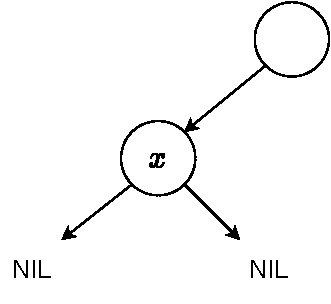
\includegraphics[scale=0.5]{img/del-leaf.ps}
  \caption{叶子节点$x$可以直接“切下”} \label{fig:del-leaf}
\end{figure}

\begin{figure}[htbp]
  \centering
  \subcaptionbox{删除$x$前}{\includegraphics[scale=0.5]{img/del-lc-before.ps}}
  \subcaptionbox{删除$x$后。$x$被“切掉”并由其左侧分支代替}{\includegraphics[scale=0.5]{img/del-lc-after.ps}} \\
  \subcaptionbox{删除$x$前}{\includegraphics[scale=0.5]{img/del-rc-before.ps}}
  \subcaptionbox{删除$x$后。$x$被“切掉”并由其右侧分支代替}{\includegraphics[scale=0.5]{img/del-rc-after.ps}}
  \caption{删除只有一个非空子分支的节点}
  \label{fig:del-1child}
\end{figure}

\begin{figure}[htbp]
  \centering
  \subcaptionbox{删除$x$前}{\includegraphics[scale=0.5]{img/del-branch-before.ps}}
  \subcaptionbox{删除$x$后。$x$被替换为右侧分支中的被“切下”的最小值}{ \includegraphics[scale=0.5]{img/del-branch-after.ps}}
  \caption{删除有两个非空分支的节点}
  \label{fig:del-branch}
\end{figure}

根据这个思路,我们定义下面的$delete$函数:

\be
\begin{array}{rcl}
delete(\nil, x) & = & \nil\\
delete(Node(T_l, k, T_r), x) & = & \begin{cases}
  x < k: & Node(delete(T_l, x), k, T_r) \\
  x > k: & Node(T_l, k, delete(T_r, x)) \\
  x = k: & del(T_l, T_r) \\
\end{cases}
\end{array}
\ee

算法先通过序关系找到待删除节点,然后调用$del$函数处理,$del$会根据情况递归调用$delete$以删除右子树中的最小值。

\be
\begin{array}{rcl}
del(\nil, T_r) & = & T_r \\
del(T_l, \nil) & = & T_l \\
del(T_l, T_r) & = & Node(T_l, y, delete(T_r, y)) \\
\end{array}
\ee

其中$y = min(T_r)$是右子树中的最小元素。下面是相应的例子程序:

\begin{Haskell}
delete Empty _ = Empty
delete (Node l k r) x | x < k = Node (delete l x) k r
                      | x > k = Node l k (delete r x)
                      | otherwise = del l r
  where
    del Empty r = r
    del l Empty = l
    del l r = let k' = min r in Node l k' (delete r k')
\end{Haskell}

如果树的高度为$h$,则删除算法的复杂度为$O(h)$。命令式算法需要在删除后,把父节点设置正确。下面的算法返回删除后树的根节点。

\begin{algorithmic}[1]
\Function{Delete}{$T, x$}
  \State $r \gets T$
  \State $x' \gets x$ \Comment{save $x$}
  \State $p \gets $ \Call{Parent}{$x$}
  \If{\Call{Left}{$x$} $= $ NIL}
    \State $x \gets $ \Call{Right}{$x$}
  \ElsIf{\Call{Right}{$x$} $= $ NIL}
    \State $x \gets $ \Call{Left}{$x$}
  \Else
    \Comment{neither children is empty}
    \State  $y \gets $ \textproc{Min}(\Call{Right}{$x$})
    \State \Call{Key}{$x$} $\gets$ \Call{Key}{$y$}
    \State Copy other satellite data from $y$ to $x$
    \If{\Call{Parent}{$y$} $\neq x$}
      \Comment{$y$ does not have left sub-tree}
      \State \textproc{Left}(\Call{Parent}{$y$}) $\gets$ \Call{Right}{$y$}
    \Else
      \Comment{$y$ is the root of the right sub-tree}
      \State \Call{Right}{$x$} $\gets$ \Call{Right}{$y$}
    \EndIf
    \If{\Call{Right}{$y$} $\neq $ NIL}
      \State \textproc{Parent}(\Call{Right}{$y$}) $\gets$ \Call{Parent}{$y$}
    \EndIf
    \State Remove $y$
    \State \Return $r$
  \EndIf
  \If{$x \neq $ NIL}
    \State \Call{Parent}{$x$} $\gets p$
  \EndIf
  \If{$p = $ NIL}
    \Comment{remove the root}
    \State $r \gets x$
  \Else
    \If{\Call{Left}{$p$} $= x'$}
      \State \Call{Left}{$p$} $\gets x$
    \Else
      \State \Call{Right}{$p$} $\gets x$
    \EndIf
  \EndIf
  \State Remove $x'$
  \State \Return $r$
\EndFunction
\end{algorithmic}

假定待删除的节点$x$不为空。算法首先记录下树的根节点、待删除的节点和它的父节点。如果$x$的任一分支为空,算法直接将$x$“切掉”。否则,如果两个子分支都不为空,我们需要先在右子树中找到最小值节点$y$。用$y$替换掉$x$中的值,同时将附加数据也替换过去。最后将原先的$y$“切掉”。我们还需要处理$y$是$x$右子树的根节点这一特殊情况。

此后还需要把之前保存的父节点重新设好。如果父节点为空,则说明要删除的节点是根节点。这种情况下,我们需要返回新的根。当父节点被设置好后,就可以安全把$x$删除了。对于高度为$h$的树,这一算法的复杂度也是$O(h)$。

\begin{Exercise}
\Question{当节点的两个分支都不为空时,存在一种对称的删除算法:用左子树的最大值替换待删除的节点,然后将此最大值的节点“切下”。编程实现这一算法。}
\end{Exercise}

\section{随机构建}
\index{二叉搜索树!随机构建}

本章给出的所有算法的复杂度都依赖于树的高度$h$。如果树非常不平衡,$O(h)$就会接近$O(n)$,因而退化为线性复杂度。反之,如果树平衡,$O(h)$接近$O(\lg n)$,算法的性能就会很好。

第三、四章将介绍两种保证二叉搜索树的平衡的方法。这里我们先给出一个简单的方法(\cite{CLRS}第265-268页):可以通过随机构建来减小不平衡性。也就是说,在构建二叉搜索树前,先通过随机函数打乱元素的次序,然后再依次插入。

\begin{Exercise}
\Question{编程实现随机构建二叉搜索树。}
\Question{如何在一棵二叉树中找到“距离最远”的两个节点?}
\end{Exercise}

\section{附录:例子代码}

包含父节点引用的二叉搜索树的例子定义:

\lstset{language=Bourbaki, frame=single}
\begin{lstlisting}
data Node<T> {
    T key
    Node<T> left
    Node<T> right
    Node<T> parent

    Node(T x) { key = x }
    Node(Node<T> l, T k, Node<T> r) {
        left = l, key = k, right = r
    }
}
\end{lstlisting}

不使用模式匹配的插入算法:

\begin{lstlisting}
Node<T> insert (Node<T> t, T x) {
    if (t == null) {
        return Node(null, x, null)
    } else if (t.key < x) {
        return Node(insert(t.left, x), t.key, t.right)
    } else {
        return Node(t.left, t.key, insert(t.right, x))
    }
}
\end{lstlisting}

消除递归的查找算法:

\begin{lstlisting}
Optional<Node<T>> lookup (Node<T> t, T x) {
    while (t != null and t.key != x) {
        if (x < t.key) {
            t = t.left
        } else {
            t = t.right
        }
    }
    return Optional(t);
}
\end{lstlisting}

迭代寻找最小元素:

\begin{lstlisting}
Optional<Node<T>> min (Node<T> t) {
    while (t != null and t.left != null) {
        t = t.left
    }
    return Optional(t);
}
\end{lstlisting}

寻找给定节点的后继:

\begin{lstlisting}
Optional<Node<T>> succ (Node<T> x) {
    if (x == null) {
        return Optional.None
    } else if (x.right != null) {
        return min(x.right)
    } else {
        p = x.parent
        while (p != null and x == p.right) {
            x = p
            p = p.parent
        }
        return Optional(p);
    }
}
\end{lstlisting}

删除节点:

\begin{lstlisting}
Node<T> delete(Node<T> t, Node<T> x) {
    if (x == null) {
        return t
    }
    root, x0, parent = t, x, x.parent
    if (x.left == null) {
        x = x.right
    } else if (x.right == null) {
        x = x.left
    } else {
        y = min(x.right)
        x.key = y.key
        if (y.parent != x) {
            y.parent.left = y.right
        } else {
            x.right = y.right
        }
        if (y.right != null) {
            y.right.parent = y.parent
        }
        return root
    if (x != null) {
        x.parent = parent
    }
    if (parent == null) {
        root = x
    } else {
        if (parent.left == x0) {
            parent.left = x
        } else {
            parent.right = x
        }
    return root
}
\end{lstlisting}

\ifx\wholebook\relax \else
\begin{thebibliography}{99}

\bibitem{CLRS}
Thomas H. Cormen, Charles E. Leiserson, Ronald L. Rivest and Clifford Stein.
``Introduction to Algorithms, Second Edition''(《算法导论》中文版). ISBN:0262032937. The MIT Press. 2001

\bibitem{Bentley}
Jon Bentley. ``Programming Pearls(2nd Edition)''(《编程珠玑》中文版). Addison-Wesley Professional; 2 edition (October 7, 1999). ISBN-13: 978-0201657883

\bibitem{okasaki-blog}
Chris Okasaki. ``Ten Years of Purely Functional Data Structures''. http://okasaki.blogspot.com/2008/02/ten-years-of-purely-functional-data.html

\bibitem{sgi-stl}
SGI. ``Standard Template Library Programmer's Guide''. http://www.sgi.com/tech/stl/

\bibitem{wiki-fold}
http://en.wikipedia.org/wiki/Foldl

\bibitem{func-composition}
http://en.wikipedia.org/wiki/Function\_composition

\bibitem{curry}
http://en.wikipedia.org/wiki/Partial\_application

\bibitem{learn-haskell}
Miran Lipovaca. ``Learn You a Haskell for Great Good! A Beginner's Guide''. the last chapter. No Starch Press; 1 edition April 2011, 400 pp. ISBN: 978-1-59327-283-8

\end{thebibliography}

\end{document}
\fi
